% =====================================================================
% main.tex
% Responsabilidad única: ensamblar el documento completo a partir de los
% módulos (preámbulo, portada y las diez secciones de ejercicios). No
% contiene desarrollo matemático ni resultados propios — solo estructura.
%
% Para compilar:  pdflatex main.tex   (dos veces, por el índice)
%             o:  latexmk -pdf main.tex
% =====================================================================
\documentclass[11pt]{article}

% =====================================================================
% preambulo.tex
% Responsabilidad única: cargar paquetes y definir configuración/estilos
% reutilizables (colores de enlaces, entornos, listas). No contiene
% contenido propio del taller — si algo del "look" del documento debe
% cambiar, este es el único archivo que hay que tocar.
% =====================================================================

\usepackage[utf8]{inputenc}
\usepackage[T1]{fontenc}
\usepackage[spanish,es-noshorthands]{babel}
\usepackage[a4paper,margin=2.5cm]{geometry}

% --- Matemáticas ------------------------------------------------------
\usepackage{amsmath}
\usepackage{amssymb}
\usepackage{amsthm}
\usepackage{mathtools}

% --- Tablas y figuras ---------------------------------------------------
\usepackage{graphicx}
\usepackage{booktabs}
\usepackage{array}
\usepackage{multirow}
\usepackage{caption}
\usepackage{float}

% --- Listas con formato a., b., c. ------------------------------------
\usepackage{enumitem}

% --- Diagramas vectoriales -----------------------------------------------
\usepackage{tikz}
\usetikzlibrary{arrows.meta, positioning, calc}
% Misma paleta usada en las figuras generadas con matplotlib (Ejercicios
% 6-8), para que los diagramas TikZ se vean como parte del mismo documento.
\definecolor{classblue}{HTML}{4C72B0}
\definecolor{classred}{HTML}{C44E52}
\definecolor{classgreen}{HTML}{55A868}

% --- Color y enlaces ----------------------------------------------------
\usepackage{xcolor}
\definecolor{urosariored}{RGB}{255,11,38} % rojo exacto muestreado del escudo
\usepackage{hyperref}
\hypersetup{
    colorlinks = true,
    linkcolor  = urosariored!75!black,
    citecolor  = urosariored!75!black,
    urlcolor   = urosariored!75!black,
    pdftitle   = {Taller 1 -- KNN y Metricas de Clasificacion},
    pdfauthor  = {Over Haider Castrillon Valencia},
}

% --- Espaciado de tablas ------------------------------------------------
\renewcommand{\arraystretch}{1.25}

% --- Pie de página institucional -----------------------------------------
% Responsabilidad de este bloque: mostrar el escudo de la Universidad del
% Rosario, pequeño, en la esquina inferior derecha de cada página del
% cuerpo del documento (la portada define su propio pie por separado en
% portada.tex, ya que \begin{titlepage} usa página sin estilo).
\usepackage{fancyhdr}
\pagestyle{fancy}
\fancyhf{}
\renewcommand{\headrulewidth}{0pt}
\renewcommand{\footrulewidth}{0pt}
\fancyfoot[C]{\thepage}
\fancyfoot[R]{
\includegraphics[height=0.42cm]{figuras/logo_urosario_icono.png}}

% --- Encabezados de subsección sin numerar, para incisos a-e -----------
\setlist[enumerate,1]{label=\alph*., leftmargin=1.6em}


\begin{document}

% =====================================================================
% portada.tex
% Responsabilidad única: presentar los datos identificativos del taller
% (título, curso, estudiante, profesor, fecha). No contiene desarrollo
% matemático ni resultados.
% =====================================================================

\begin{titlepage}
    \centering
    \vspace*{2cm}

    {\LARGE \textbf{Taller 1 --- KNN y Métricas de Clasificación}}\\[0.6cm]
    {\large Aprendizaje Automático de Máquina I}\\[0.15cm]
    {\large Semestre 2026-2}\\[1.6cm]

    \rule{0.8\textwidth}{0.4pt}\\[0.9cm]

    \begin{tabular}{rl}
        \textbf{Estudiante:}    & Over Haider Castrillón Valencia \\[0.35em]
        \textbf{Programa:}      & Maestría en Matemáticas y Ciencias de la Computación \\[0.35em]
        \textbf{Profesor:}      & Daniel Felipe Rambaut Lemus \\[0.35em]
        \textbf{Modalidad:}     & Individual \\[0.35em]
        \textbf{Fecha:}         & \today \\
    \end{tabular}

    \vfill
    
\includegraphics[width=2.6cm]{figuras/logo_urosario.png}
\end{titlepage}


\tableofcontents
\newpage

% ---------------------------------------------------------------------
% Parte I — Componente teórico-matemático
% ---------------------------------------------------------------------
\section{Componente teórico-matemático}
% =====================================================================
% ejercicio01.tex
% Responsabilidad única: demostrar que \hat p_k(x) es una proporción,
% derivar la regla de decisión por umbral 1/2, resolver los dos casos
% numéricos (k=5 y k=7), y justificar por qué k impar evita empates.
% =====================================================================
\subsection{Ejercicio 1 --- Fundamento probabilístico de KNN}

Sea un conjunto de entrenamiento $D=\{(x_i,y_i)\}_{i=1}^n$, con
$x_i\in\mathbb{R}^d$, $y_i\in\{0,1\}$. Para una nueva observación $x$,
sea $N_k(x)$ el conjunto de sus $k$ vecinos más cercanos, y defínase

\[
    \hat p_k(x) = \frac{1}{k}\sum_{x_i \in N_k(x)} y_i .
\]

\begin{enumerate}

\item \textbf{$\hat p_k(x)$ es una proporción.}
Dado que $y_i\in\{0,1\}$, cada etiqueta funciona como una variable
indicadora, de forma que $y_i=1$ aporta exactamente una unidad a la
suma cuando el vecino pertenece a la clase positiva, mientras que
$y_i=0$ no aporta nada, por lo tanto,
\[
    \sum_{x_i\in N_k(x)} y_i = \#\{x_i\in N_k(x) : y_i = 1\} = m,
\]
es decir, la sumatoria cuenta literalmente cuántos de los $k$ vecinos
son positivos sin que los negativos alteren el resultado, y al dividir
entre $k$ se obtiene $\hat p_k(x)=m/k$, que corresponde exactamente a
la definición frecuentista de una proporción (casos favorables sobre
casos totales), quedando así demostrado que $\hat p_k(x)$ es la
proporción de vecinos de clase positiva.

\item \textbf{El umbral $\tfrac12$ como regla de mayoría.}
KNN asigna a $x$ la clase mayoritaria entre sus $k$ vecinos, de forma
que, si $m$ es el número de vecinos positivos, entonces $k-m$ es el de
negativos, y la clase 1 es mayoritaria cuando $m > k-m$, lo cual
equivale a $2m>k$, es decir, a $m/k>\tfrac12$ (y como
$\hat p_k(x)=m/k$, esta condición es exactamente
$\hat p_k(x) > \tfrac12$), con lo cual el umbral no se impone
arbitrariamente, sino que es la traducción algebraica directa de la
regla ``la clase con más votos gana''.

\item \textbf{Caso $k=5$, etiquetas $\{1,0,1,1,0\}$.}
\[
    m = 1+0+1+1+0 = 3, \qquad \hat p_k(x) = \frac{3}{5} = 0.6 > 0.5
    \;\Longrightarrow\; \text{KNN predice la \textbf{clase 1}.}
\]

\item \textbf{Caso $k=7$, etiquetas $\{0,0,1,0,1,1,0\}$.}
\[
    m = 0+0+1+0+1+1+0 = 3, \qquad \hat p_k(x) = \frac{3}{7} \approx 0.4286 < 0.5
    \;\Longrightarrow\; \text{KNN predice la \textbf{clase 0}.}
\]

\item \textbf{Por qué $k$ impar evita empates.}
Un empate ocurre cuando $m = k-m$, es decir, cuando $k=2m$, y esta
igualdad exige que $k$ sea par (porque $2m$ es siempre un número par
para cualquier entero $m$), de modo que si $k$ es impar no existe
ningún entero $m$ que satisfaga $k=2m$, y el empate resulta
matemáticamente imposible, que es justo lo que se observó en los
incisos c y d, donde al ser $k$ impar en ambos casos, $\hat p_k(x)$
nunca cae exactamente en $0.5$ y siempre hay una clase estrictamente
mayoritaria.

\end{enumerate}

\begin{figure}[H]
\centering
\begin{tikzpicture}[every node/.style={font=\small}]

\draw[dashed, gray!60, thick] (0,0) circle (2.4);
\node[gray!55] at (2.95,1.55) {$N_5(x)$};

\draw[gray!45] (0,0) -- (90:2);
\draw[gray!45] (0,0) -- (162:1.8);
\draw[gray!45] (0,0) -- (234:2.1);
\draw[gray!45] (0,0) -- (306:1.9);
\draw[gray!45] (0,0) -- (18:2.2);

\node[draw=black, fill=black, rectangle, minimum size=8pt, inner sep=0pt] (x) at (0,0) {};
\node[below=2pt] at (0,-0.22) {$x$};

\node[draw=black, fill=classred,  circle, minimum size=10pt, inner sep=0pt] (n1) at (90:2)   {};
\node[draw=black, fill=classblue, circle, minimum size=10pt, inner sep=0pt] (n2) at (162:1.8) {};
\node[draw=black, fill=classred,  circle, minimum size=10pt, inner sep=0pt] (n3) at (234:2.1) {};
\node[draw=black, fill=classred,  circle, minimum size=10pt, inner sep=0pt] (n4) at (306:1.9) {};
\node[draw=black, fill=classblue, circle, minimum size=10pt, inner sep=0pt] (n5) at (18:2.2)  {};

\node[draw=black, fill=classred, circle, minimum size=10pt, inner sep=0pt] (lr) at (3.7,0.55) {};
\node[right=5pt] at (lr) {clase 1};
\node[draw=black, fill=classblue, circle, minimum size=10pt, inner sep=0pt] (lb) at (3.7,-0.05) {};
\node[right=5pt] at (lb) {clase 0};
\node[draw=black, fill=black, rectangle, minimum size=8pt, inner sep=0pt] (lx) at (3.7,-0.65) {};
\node[right=5pt] at (lx) {consulta $x$};

\node[align=center, text width=8.6cm] at (0.9,-3.05)
  {\textbf{3 votos de clase 1} contra \textbf{2 votos de clase 0}
   $\Rightarrow\ \hat p_5(x)=\dfrac{3}{5}=0.6 > \dfrac12$
   $\Rightarrow$ predicción: \textbf{clase 1}};

\end{tikzpicture}
\caption{Votación de KNN para el ejemplo del inciso c ($k=5$, etiquetas
$\{1,0,1,1,0\}$): cada punto de color es uno de los 5 vecinos más
cercanos a $x$, y la clase mayoritaria entre ellos determina la
predicción.}
\end{figure}

% =====================================================================
% ejercicio02.tex
% Responsabilidad única: calcular y comparar d_E y d_M sobre tres puntos
% dados, y demostrar la desigualdad general d_E(A,B) <= d_M(A,B).
% =====================================================================
\subsection{Ejercicio 2 --- Distancia euclidiana vs. Manhattan}

Sean $A=(a_1,a_2)$ y $B=(b_1,b_2)$, con

\[
    d_E(A,B) = \sqrt{(a_1-b_1)^2+(a_2-b_2)^2}, \qquad
    d_M(A,B) = |a_1-b_1|+|a_2-b_2|.
\]

Se consideran los puntos $A=(2,3)$, $B=(7,7)$, $C=(5,2)$.

\begin{enumerate}

\item
\[
    d_E(A,B) = \sqrt{(2-7)^2+(3-7)^2} = \sqrt{25+16} = \sqrt{41} \approx 6.4031
\]

\item
\[
    d_M(A,B) = |2-7|+|3-7| = 5+4 = 9
\]

\item
\[
    d_E(A,C) = \sqrt{(2-5)^2+(3-2)^2} = \sqrt{10} \approx 3.1623,
    \qquad
    d_M(A,C) = |2-5|+|3-2| = 4
\]

\item \textbf{Vecino más cercano de $A$.}
{\sloppy Al comparar $d_E(A,B)\approx 6.40$ con $d_E(A,C)\approx 3.16$,
y $d_M(A,B)=9$ con $d_M(A,C)=4$, resulta claro que en ambos casos
\textbf{C} es el vecino más cercano, de forma que aquí las dos
métricas coinciden en su conclusión, aunque esto no está garantizado
en general, pues nada impide construir puntos donde Euclidiana y
Manhattan discrepen sobre cuál es el vecino más cercano.\par}

\item \textbf{Demostración de $d_E(A,B)\le d_M(A,B)$.}
Partiendo de la expresión sugerida y expandiendo el cuadrado del lado
izquierdo,
\[
    (|a_1-b_1|+|a_2-b_2|)^2 = (a_1-b_1)^2 + 2|a_1-b_1||a_2-b_2| + (a_2-b_2)^2 ,
\]
y como el término cruzado $2|a_1-b_1||a_2-b_2|$ es siempre no negativo
(por ser producto de valores absolutos), se cumple que
\[
    (|a_1-b_1|+|a_2-b_2|)^2 \;\ge\; (a_1-b_1)^2+(a_2-b_2)^2,
\]
es decir, $d_M(A,B)^2 \ge d_E(A,B)^2$, y dado que ambas distancias son
cantidades no negativas, al tomar raíz cuadrada la desigualdad se
preserva:
\[
    d_M(A,B) \ge d_E(A,B) \quad\Longleftrightarrow\quad d_E(A,B)\le d_M(A,B).
\]
La igualdad solo se alcanza cuando $|a_1-b_1||a_2-b_2|=0$, es decir,
cuando los puntos difieren en una única coordenada (geométricamente,
cuando el desplazamiento es puramente horizontal o vertical).

\end{enumerate}

\begin{figure}[H]
\centering
\begin{tikzpicture}[scale=0.68, every node/.style={font=\small}]

\draw[step=1, gray!22, thin] (0,0) grid (8,8);
\draw[-{Stealth[length=6pt]}] (-0.4,0) -- (8.6,0) node[right] {$x_1$};
\draw[-{Stealth[length=6pt]}] (0,-0.4) -- (0,8.6) node[above] {$x_2$};

\coordinate (A) at (2,3);
\coordinate (B) at (7,7);

\draw[very thick, classblue] (A) -- (7,3) -- (B);
\draw[very thick, classred] (A) -- (B);

\node[draw=black, fill=black, circle, minimum size=5pt, inner sep=0pt] at (A) {};
\node[below left=1pt and -2pt] at (A) {$A=(2,3)$};
\node[draw=black, fill=black, circle, minimum size=5pt, inner sep=0pt] at (B) {};
\node[above right=1pt and -2pt] at (B) {$B=(7,7)$};

\node[classred, fill=white, inner sep=1pt] at (3.35,5.05) {$d_E\approx 6.40$};
\node[classblue] at (4.5,2.55) {$d_M=9$};

\end{tikzpicture}
\caption{Trayecto directo (Euclidiana, rojo) frente al trayecto en
escalera (Manhattan, azul) entre $A$ y $B$: la escalera nunca puede ser
más corta que la línea recta, lo que ilustra geométricamente por qué
$d_E \le d_M$.}
\end{figure}

% =====================================================================
% ejercicio03.tex
% Responsabilidad única: mostrar, con un ejemplo numérico y su
% generalización algebraica, por qué una variable de escala mayor
% domina la distancia euclidiana cuando no se estandariza — es la base
% conceptual que se retoma empíricamente en el Ejercicio 7.
% =====================================================================
\subsection{Ejercicio 3 --- Efecto de la escala sobre la distancia}

Se consideran los puntos $A=(20,1000)$, $B=(25,1200)$, $C=(40,1010)$.

\begin{enumerate}

\item \textbf{Distancias en escala original.}
\[
    d(A,B) = \sqrt{(20-25)^2+(1000-1200)^2} = \sqrt{25+40000} = \sqrt{40025} \approx 200.06
\]
\[
    d(A,C) = \sqrt{(20-40)^2+(1000-1010)^2} = \sqrt{400+100} = \sqrt{500} \approx 22.36
\]

\item \textbf{Vecino más cercano.}
Como $d(A,C)\approx 22.36$ es mucho menor que $d(A,B)\approx 200.06$,
el punto \textbf{C} es el vecino más cercano a $A$.

\item \textbf{Distancias tras dividir la segunda variable entre 100.}
Con $A'=(20,10)$, $B'=(25,12)$, $C'=(40,10.1)$:
\[
    d(A',B') = \sqrt{5^2+2^2} = \sqrt{29} \approx 5.385
\]
\[
    d(A',C') = \sqrt{20^2+0.1^2} = \sqrt{400.01} \approx 20.0002
\]

\item \textbf{¿Cambió el vecino más cercano?}
Sí, ahora $d(A',B')\approx 5.39 < d(A',C')\approx 20.00$ así que el
vecino más cercano pasó a ser \textbf{B}, el punto opuesto al de antes
de reescalar pero esto tiene una explicación directa: En la escala
original la segunda variable (diferencias en centenas) dominaba por
completo el cálculo, mientras que al dividirla entre 100 su diferencia
se vuelve comparable a la de la primera variable y esta última antes
irrelevante, ahora pasa a determinar la distancia.

\item \textbf{Por qué una escala mayor domina la distancia.}
En la expresión general
\[
    d(x,z) = \sqrt{\sum_{j=1}^{d} (x_j-z_j)^2},
\]
cada variable contribuye a través del cuadrado de su diferencia, de
modo que si la variable $j$ tiene un rango considerablemente mayor al
de las demás (como la segunda coordenada (ordenada) de este ejercicio en orden de miles y no decenas), $(x_j-z_j)^2$ será en términos absolutos,
mucho mayor que los demás términos, de forma que tanto la suma como,
en consecuencia, la distancia total terminan determinadas casi
exclusivamente por esa variable sin importar si conceptualmente es la
más relevante para el problema, este es precisamente el motivo por
el cual antes de aplicar un algoritmo basado en distancias como KNN,
se recomienda estandarizar o normalizar las variables.

\end{enumerate}

\begin{figure}[H]
\centering
\begin{tikzpicture}[every node/.style={font=\footnotesize}]

% ===== Panel 1: antes de estandarizar =====
\begin{scope}
\draw[gray!50] (0,0) -- (3.5,0);
\pgfmathsetmacro{\hA}{200.06*0.011}
\pgfmathsetmacro{\hC}{22.36*0.011}
\draw[fill=gray!45, draw=gray!70] (0.15,0) rectangle (0.85,\hA);
\draw[fill=classgreen, draw=black] (2.15,0) rectangle (2.85,\hC);
\node at (0.5,\hA+0.28) {$200.06$};
\node[classgreen, font=\scriptsize\bfseries] at (2.5,\hC+0.32) {$\star$ más cercano};
\node at (2.5,\hC+0.62) {$22.36$};
\node at (0.5,-0.35) {$d(A,B)$};
\node at (2.5,-0.35) {$d(A,C)$};
\node[align=center, font=\small\bfseries] at (1.5,-1.0) {Antes de estandarizar};
\end{scope}

% ===== Panel 2: despues de estandarizar =====
\begin{scope}[shift={(5.6,0)}]
\draw[gray!50] (0,0) -- (3.5,0);
\pgfmathsetmacro{\hBp}{5.385*0.11}
\pgfmathsetmacro{\hCp}{20.0002*0.11}
\draw[fill=classgreen, draw=black] (0.15,0) rectangle (0.85,\hBp);
\draw[fill=gray!45, draw=gray!70] (2.15,0) rectangle (2.85,\hCp);
\node[classgreen, font=\scriptsize\bfseries] at (0.5,\hBp+0.32) {$\star$ más cercano};
\node at (0.5,\hBp+0.62) {$5.385$};
\node at (2.5,\hCp+0.28) {$20.0002$};
\node at (0.5,-0.35) {$d(A',B')$};
\node at (2.5,-0.35) {$d(A',C')$};
\node[align=center, font=\small\bfseries] at (1.5,-1.0) {Después de estandarizar};
\end{scope}

\end{tikzpicture}
\caption{Cambio del vecino más cercano de $A$ tras dividir la segunda
variable entre 100 (cada panel usa su propia escala vertical, ya que
las magnitudes antes y después no son comparables): pasa de ser $C$ a
ser $B$.}
\end{figure}

% =====================================================================
% ejercicio04.tex
% Responsabilidad única: extraer TP/TN/FP/FN de una matriz de confusión
% dada, calcular Accuracy/Precision/Recall/F1, y demostrar la forma
% alternativa de F1 en función únicamente de TP, FP y FN.
% =====================================================================
\subsection{Ejercicio 4 --- Matriz de confusión y métricas básicas}

\begin{table}[H]
\centering
\begin{tabular}{cc|cc}
    & & \multicolumn{2}{c}{\textbf{Predicho}} \\
    & & $\hat Y = 0$ & $\hat Y = 1$ \\
    \hline
    \multirow{2}{*}{\textbf{Real}}
    & $Y=0$ & 850 & 100 \\
    & $Y=1$ & 20  & 30  \\
\end{tabular}
\caption{Matriz de confusión del Ejercicio 4.}
\end{table}

\begin{enumerate}

\item \textbf{Identificación de $TP,TN,FP,FN$.}
Leyendo las filas como clase real y las columnas como clase predicha,
se identifica que $TN=850$ (real 0, predicho 0), $FP=100$ (real 0,
predicho 1), $FN=20$ (real 1, predicho 0) y $TP=30$ (real 1, predicho 1).

\item \textbf{Accuracy.}
\[
    \text{Accuracy} = \frac{TP+TN}{TP+TN+FP+FN} = \frac{30+850}{1000} = 0.88
\]

\item \textbf{Precision.}
\[
    \text{Precision} = \frac{TP}{TP+FP} = \frac{30}{130} = \frac{3}{13} \approx 0.2308
\]

\item \textbf{Recall.}
\[
    \text{Recall} = \frac{TP}{TP+FN} = \frac{30}{50} = 0.6
\]

\item \textbf{F1.}
\[
    F1 = 2\cdot\frac{\text{Precision}\cdot\text{Recall}}{\text{Precision}+\text{Recall}}
       = 2\cdot\frac{(3/13)(3/5)}{3/13+3/5}
       = 2\cdot\frac{9/65}{54/65}
       = \frac{18}{54} = \frac13 \approx 0.3333
\]

\item \textbf{Demostración algebraica de $F1 = \dfrac{2TP}{2TP+FP+FN}$.}

Se parte de las definiciones $P = \dfrac{TP}{TP+FP}$ y $R = \dfrac{TP}{TP+FN}$.

Primero se calcula el producto $P\cdot R$:
\[
    P\cdot R = \frac{TP^2}{(TP+FP)(TP+FN)}.
\]

Luego se calcula la suma $P+R$, llevándola a un denominador común:
\[
    P + R = \frac{TP(TP+FN)+TP(TP+FP)}{(TP+FP)(TP+FN)} = \frac{TP\,(2TP+FP+FN)}{(TP+FP)(TP+FN)}.
\]

Sustituyendo ambas expresiones en $F1 = 2\cdot\dfrac{P\cdot R}{P+R}$,
el denominador común $(TP+FP)(TP+FN)$ se cancela:
\[
    F1 = 2\cdot\frac{TP^2}{TP\,(2TP+FP+FN)} = \frac{2TP}{2TP+FP+FN}.
\]

Verificación numérica:
\[
    \frac{2(30)}{2(30)+100+20} = \frac{60}{180} = \frac13,
\]
idéntico al resultado del inciso e.

\end{enumerate}

% =====================================================================
% ejercicio05.tex
% Responsabilidad única: contrastar dos matrices de confusión bajo las
% cuatro métricas estándar y bajo un costo asimétrico L=FP+5FN,
% evidenciando que "mejor Accuracy" no implica "menor costo".
% =====================================================================
\subsection{Ejercicio 5 --- Comparación de dos modelos y costo de clasificación}

\begin{table}[H]
\centering
\begin{minipage}{0.45\textwidth}
\centering
\begin{tabular}{cc|cc}
    & & \multicolumn{2}{c}{\textbf{Predicho}} \\
    & & $\hat Y=0$ & $\hat Y=1$ \\
    \hline
    \multirow{2}{*}{\textbf{Real}} & $Y=0$ & 900 & 50 \\
    & $Y=1$ & 30 & 20 \\
\end{tabular}
\caption*{Modelo A}
\end{minipage}
\hfill
\begin{minipage}{0.45\textwidth}
\centering
\begin{tabular}{cc|cc}
    & & \multicolumn{2}{c}{\textbf{Predicho}} \\
    & & $\hat Y=0$ & $\hat Y=1$ \\
    \hline
    \multirow{2}{*}{\textbf{Real}} & $Y=0$ & 850 & 100 \\
    & $Y=1$ & 10 & 40 \\
\end{tabular}
\caption*{Modelo B}
\end{minipage}
\caption{Matrices de confusión de los dos modelos comparados.}
\end{table}

\begin{enumerate}

\item \textbf{Métricas de cada modelo.}
Modelo A ($TN=900,FP=50,FN=30,TP=20$):
\[
    \text{Acc}_A = 0.92, \quad
    \text{Prec}_A = \tfrac{20}{70}\approx 0.2857, \quad
    \text{Rec}_A = 0.4, \quad
    F1_A = \tfrac13 \approx 0.3333.
\]
Modelo B ($TN=850,FP=100,FN=10,TP=40$):
\[
    \text{Acc}_B = 0.89, \quad
    \text{Prec}_B = \tfrac{40}{140}\approx 0.2857, \quad
    \text{Rec}_B = 0.8, \quad
    F1_B = \tfrac{8}{19} \approx 0.4211.
\]

\item \textbf{Costo $L=FP+5FN$.}
\[
    L_A = 50+5(30) = 200, \qquad L_B = 100+5(10) = 150.
\]

\item \textbf{Mayor Accuracy:} el Modelo A ($0.92 > 0.89$).

\item \textbf{Mayor Recall:} el Modelo B ($0.8 > 0.4$), por amplio margen.

\item \textbf{Menor costo:} el Modelo B ($150 < 200$).

\item \textbf{El modelo de mayor Accuracy no minimiza el costo.}
El Modelo A tiene mayor Accuracy pero un mayor coste asociado que el
Modelo B, esto sucede porque lo que hace el Accuracy es ponderar todos
los errores por igual, mientras que $L$ pondera cada falso negativo
cinco veces más que cada falso positivo: el Modelo A minimiza el
número total de errores ($80$ en vez de $110$), pero comete más falsos
negativos ($30$ y no $10$), que son los más costosos, mientras que el
Modelo B sí compensa con más falsos positivos ($100$ en vez de $50$),
los que son baratos. Cuando los dos tipos de error tienen consecuencias
distintas, elegir un modelo únicamente por el Accuracy puede ser una
decisión subóptima enmarcada en el costo real del negocio.

\end{enumerate}


\newpage
% ---------------------------------------------------------------------
% Parte II — Componente práctico-computacional
% ---------------------------------------------------------------------
\section{Componente práctico-computacional}
\label{sec:practico}

\noindent Los ejercicios 6 a 10 se desarrollaron en Python sobre el
conjunto de datos \emph{Give Me Some Credit} (150.000 observaciones);
el notebook reproducible correspondiente se entrega por separado (en
formato \texttt{.ipynb}) produciendo todos los valores y figuras citados en esta sección.

% =====================================================================
% ejercicio06.tex
% Responsabilidad única: documentar el diagnóstico del dataset, el
% balance de clases, la estrategia de imputación y la partición
% train/test. Los números provienen de la ejecución real del notebook
% adjunto (Taller_1_KNN_Notebook.ipynb).
% =====================================================================
\subsection{Ejercicio 6 --- Exploración inicial y preparación de datos}

\subsubsection*{a--c. Carga del dataset y diagnóstico general}

El conjunto de datos \emph{Give Me Some Credit} contiene 150.000
observaciones y 11 variables (10 predictoras más la variable objetivo
\texttt{SeriousDlqin2yrs}) de las cuales 6 son de tipo entero
[\texttt{int64}], 4 de tipo decimal [\texttt{float64}] y solo dos
presentan valores faltantes: \texttt{MonthlyIncome} (29.731 faltantes,
$19.82\%$) y \texttt{NumberOfDependents} (3.924 faltantes, $2.62\%$),
mientras que el resto de variables no tiene ningún faltante.

\subsubsection*{d. Balance de clases}

\begin{table}[H]
\centering
\begin{tabular}{lrr}
\toprule
Clase & $n$ & \% \\
\midrule
0 (no incumple) & 139.974 & 93.32 \\
1 (incumple)     &  10.026 &  6.68 \\
\bottomrule
\end{tabular}
\caption{Distribución de la variable objetivo \texttt{SeriousDlqin2yrs}.}
\end{table}

Casi 14 casos negativos por cada positivo: Un modelo trivial que
siempre prediga la clase 0 ya alcanzaría cerca de $93\%$ de Accuracy
sin ser útil en la práctica, de modo que la Precision, Recall y F1 sobre
la clase 1 serán las métricas que realmente den informen del desempeño.

\subsubsection*{e. Gráfica}

\begin{figure}[H]
    \centering
    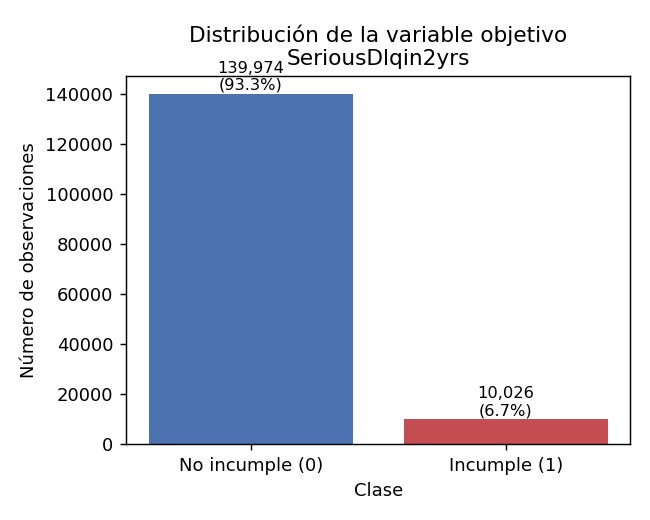
\includegraphics[width=0.55\textwidth]{figuras/ex6_distribucion_target.png}
    \caption{Distribución de la variable objetivo.}
\end{figure}

\subsubsection*{f. Tratamiento de valores faltantes}

Se imputó con la \textbf{mediana} de cada variable en lugar de la
media ya que ambas variables con faltantes tienen colas largas hacia
la derecha (unos pocos ingresos o números de dependientes
extremadamente altos que arrastrarían la media), la mediana resulta
mucho más robusta frente a esos valores atípicos, usando como
referencia \texttt{MonthlyIncome}\,$=5.400$ y
\texttt{NumberOfDependents}\,$=0$.

\subsubsection*{g. Partición 80/20 estratificada}

\begin{table}[H]
\centering
\begin{tabular}{lrrrr}
\toprule
Conjunto & Clase 0 ($n$) & Clase 0 (\%) & Clase 1 ($n$) & Clase 1 (\%) \\
\midrule
Entrenamiento (120.000) & 111.979 & 93.32 & 8.021 & 6.68 \\
Prueba (30.000)         &  27.995 & 93.32 & 2.005 & 6.68 \\
\bottomrule
\end{tabular}
\caption{Distribución de clases en entrenamiento y prueba.}
\end{table}

Se usó \texttt{train\_test\_split(X, y, test\_size=0.2, stratify=y,
random\_state=42)} (la estratificación busca mantener la proporción de
clases prácticamente idéntica entre \emph{train} y \emph{test}),
evitando que el azar de la partición produzca un subconjunto con una
tasa de incumplimiento notablemente distinta a la del conjunto
completo (lo cual sesgaría la evaluación).

% =====================================================================
% ejercicio07.tex
% Responsabilidad única: comparar el efecto de estandarizar las
% variables sobre un mismo modelo KNN (k=5), y justificar la elección
% de modelo con base en las métricas obtenidas.
% =====================================================================
\subsection{Ejercicio 7 --- KNN con $k=5$: sin escalar vs. estandarizado}

\begin{table}[H]
\centering
\begin{tabular}{lrrrr}
\toprule
Modelo & Accuracy & Precision & Recall & F1 \\
\midrule
Sin escalamiento & 0.9326 & 0.4224 & 0.0244 & 0.0462 \\
Estandarizado     & 0.9329 & 0.4936 & 0.1357 & 0.2128 \\
\bottomrule
\end{tabular}
\caption{Comparación $k=5$, sin escalar vs. estandarizado.}
\end{table}

\begin{figure}[H]
    \centering
    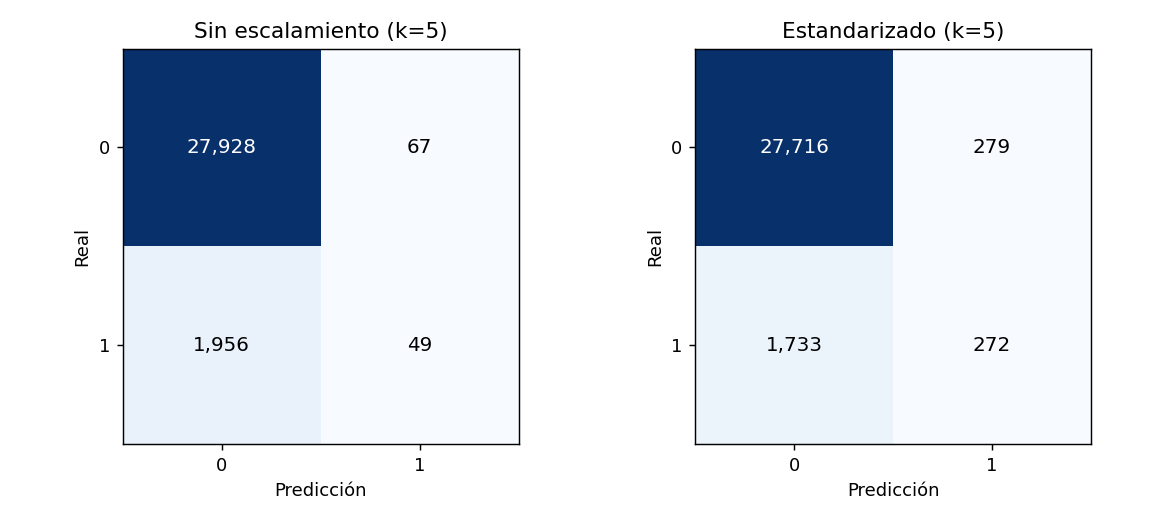
\includegraphics[width=0.85\textwidth]{figuras/ex7_matrices_confusion.png}
    \caption{Matrices de confusión, $k=5$.}
\end{figure}

\begin{enumerate}

\item \textbf{¿Cambió el desempeño tras estandarizar?}
Sí, y de forma sustancial en la capacidad de detectar la clase
positiva: el Accuracy apenas se mueve ($0.9326\to0.9329$), pero el
Recall se multiplica por casi $5.5$ veces ($0.0244\to0.1357$) y el F1
por más de $4.5$ veces ($0.0462\to0.2128$).

\item \textbf{Métrica con el cambio más importante.}
El \textbf{Recall}, y esto es consistente con lo demostrado en el
Ejercicio 3e, pues sin estandarizar las variables como
\texttt{MonthlyIncome} o \texttt{DebtRatio} (con rangos de miles)
dominan el cálculo de distancias por encima de \texttt{age} o
\texttt{NumberOfDependents} (con rangos de decenas o unidades), y el
modelo termina casi ignorando estas últimas, mientras que al
estandarizar todas aportan en una escala comparable y el modelo pasa
de detectar apenas 49 de los 2.005 incumplimientos reales a detectar
272 de esos mismos 2.005.

\item \textbf{Modelo elegido.}
Se recomienda el modelo \textbf{estandarizado}, ya que el Accuracy es
prácticamente igual pero el Recall y el F1 son considerablemente
superiores, y en un problema de riesgo crediticio, donde no detectar
un incumplimiento suele costar más que lanzar una alerta equivocada
(ver Ejercicio 10), esa mejora resulta preferible en casi cualquier
escenario de negocio razonable.

\end{enumerate}

% =====================================================================
% ejercicio08.tex
% Responsabilidad única: barrer distintos valores de k sobre los datos
% estandarizados y analizar el trade-off entre Accuracy, Recall y F1.
% =====================================================================
\subsection{Ejercicio 8 --- Efecto del número de vecinos $k$}

\begin{table}[H]
\centering
\begin{tabular}{rrrrr}
\toprule
$k$ & Accuracy & Precision & Recall & F1 \\
\midrule
1  & 0.9044 & 0.2496 & 0.2144 & \textbf{0.2307} \\
3  & 0.9276 & 0.3978 & 0.1621 & 0.2303 \\
5  & 0.9329 & 0.4936 & 0.1357 & 0.2128 \\
7  & 0.9345 & 0.5412 & 0.1277 & 0.2066 \\
9  & \textbf{0.9350} & 0.5652 & 0.1167 & 0.1935 \\
11 & 0.9346 & 0.5583 & 0.1027 & 0.1735 \\
15 & 0.9343 & 0.5549 & 0.0883 & 0.1523 \\
21 & 0.9348 & 0.5863 & 0.0813 & 0.1428 \\
\bottomrule
\end{tabular}
\caption{Métricas por valor de $k$ (datos estandarizados).}
\end{table}

\begin{figure}[H]
    \centering
    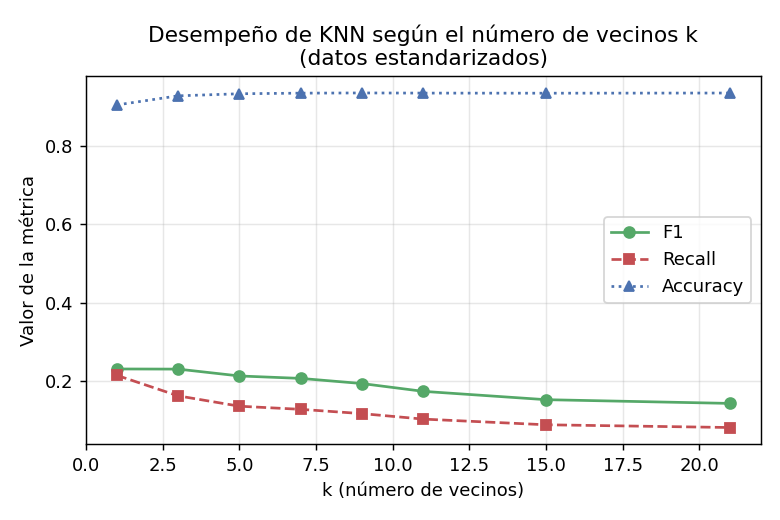
\includegraphics[width=0.7\textwidth]{figuras/ex8_k_vs_metricas.png}
    \caption{Desempeño de KNN según el número de vecinos $k$.}
\end{figure}

\begin{enumerate}

\item \textbf{Mejor F1:} $k=1$ ($F1=0.2307$).

\item \textbf{Mejor Recall:} $k=1$ ($\text{Recall}=0.2144$).

\item \textbf{Mejor Accuracy:} $k=9$ ($\text{Accuracy}=0.9350$).

\item \textbf{¿Coinciden los tres criterios en el mismo modelo?}
No, pues F1 y Recall se maximizan en $k=1$ mientras que Accuracy se
maximiza en $k=9$, y esto tiene una razón de fondo: Al aumentar $k$ el
modelo promedia sobre vecindarios cada vez más grandes que, dado el
fuerte desbalance de clases ($93\%/7\%$), terminan dominados por
vecinos de la clase mayoritaria, empujando las predicciones hacia la
clase 0 y sacrificando Recall a cambio de un Accuracy apenas mayor,
mientras que $k=1$, al fijarse solo en el vecino más próximo, es mucho
más sensible a los pocos vecinos positivos cercanos, favoreciendo el
Recall aunque a costa de una mayor varianza (más falsos positivos,
como en el Ejercicio 10).

\end{enumerate}

% =====================================================================
% ejercicio09.tex
% Responsabilidad única: comparar, para los tres mejores k según F1 del
% Ejercicio 8, el efecto de cambiar la métrica de distancia.
% =====================================================================
\subsection{Ejercicio 9 --- Distancia Euclidiana vs. Manhattan}

Se comparan los tres mejores valores de $k$ según F1 obtenidos en el
Ejercicio 8: $k=1,3,5$.

\begin{table}[H]
\centering
\begin{tabular}{rlrrrr}
\toprule
$k$ & Distancia & Accuracy & Precision & Recall & F1 \\
\midrule
1 & Euclidiana & 0.9044 & 0.2496 & 0.2144 & \textbf{0.2307} \\
1 & Manhattan  & 0.9054 & 0.2518 & 0.2105 & 0.2293 \\
3 & Euclidiana & 0.9276 & 0.3978 & 0.1621 & 0.2303 \\
3 & Manhattan  & 0.9283 & 0.4000 & 0.1466 & 0.2146 \\
5 & Euclidiana & 0.9329 & 0.4936 & 0.1357 & 0.2128 \\
5 & Manhattan  & 0.9329 & 0.4921 & 0.1237 & 0.1977 \\
\bottomrule
\end{tabular}
\caption{Euclidiana vs. Manhattan para $k \in \{1,3,5\}$.}
\end{table}

\begin{enumerate}

\item \textbf{¿La métrica modifica el desempeño?}
Sí, pero de forma mucho más discreta que la estandarización o que $k$,
y sin un patrón del todo consistente, pues para $k=1$ y $k=3$ Manhattan
da Accuracy y Precision levemente superiores pero Recall y F1
levemente inferiores a Euclidiana, mientras que para $k=5$ ocurre lo
contrario y la Euclidiana iguala o supera a Manhattan en las cuatro
métricas (obsérvese la Precision de $0.4936$ para Euclidiana y no
$0.4921$ como en la Manhattan), aunque en ningún caso la diferencia entre
métricas supera $1.5$ puntos porcentuales, muy por debajo del efecto
de estandarizar o de cambiar $k$.

\item \textbf{Mayor F1:} $k=1$, Euclidiana ($F1=0.2307$).

\item \textbf{Mayor Recall:} $k=1$, Euclidiana ($\text{Recall}=0.2144$).

\item \textbf{¿Coinciden F1 y Recall en la misma configuración?}
Sí, ambas apuntan a $k=1$ con distancia euclidiana, aunque vale la pena
matizar dicha coincidencia ya que los tres valores de $k$ comparados
aquí ya fueron preseleccionados por ranking de F1 en el Ejercicio 8, y
en este dataset el Recall resulta monótonamente decreciente en $k$ ($\uparrow \text{k}$, $\downarrow \text{Recall}$), así que el ranking de F1 y el de Recall casi
tenían que coincidir dentro de ese subconjunto de tres, por lo que no
es del todo una confirmación independiente. Dicho esto, el mecanismo
de fondo sí es real, pues a diferencia del trade-off marcado entre
$k=[1,9]$ del Ejercicio 8, aquí cambiar la métrica de distancia no
altera lo suficiente cuál vecino es ``más cercano'' como para invertir
el orden de los modelos, ya que con los datos ya estandarizados la
diferencia entre penalizar cuadráticamente (Euclidiana) o linealmente
(Manhattan) las diferencias por variable resulta menor que la que
introduce cambiar $k$.

\end{enumerate}

% =====================================================================
% ejercicio10.tex
% Responsabilidad única: seleccionar y comparar tres modelos bajo un
% costo de negocio asimétrico (L=FP+5FN), y traducir el resultado en
% una recomendación de negocio justificada.
% =====================================================================
\subsection{Ejercicio 10 --- Análisis final y costo de negocio}

Se comparan tres modelos representativos: El de mejor F1/Recall
($k=1$, Euclidiana, estandarizado), el de mejor Accuracy ($k=9$,
Euclidiana, estandarizado), y el modelo base sin estandarizar ($k=5$,
Ejercicio 7).

\begin{table}[H]
\centering
\small
\begin{tabular}{lrrrrrr}
\toprule
Modelo & $k$ & FP & FN & Recall & F1 & Costo $L$ \\
\midrule
Modelo 1 (mejor F1/Recall)          & 1 & 1.293 & 1.575 & 0.2144 & 0.2307 & \textbf{9.168} \\
Modelo 2 (mejor Accuracy)           & 9 &   180 & 1.771 & 0.1167 & 0.1935 & \textbf{9.035} \\
Modelo 3 (base, sin estandarizar)   & 5 &    67 & 1.956 & 0.0244 & 0.0462 & \textbf{9.847} \\
\bottomrule
\end{tabular}
\caption{Comparación final de modelos, con $L = FP + 5FN$.}
\end{table}

\begin{enumerate}

\item \textbf{¿El modelo de mayor Accuracy es también el de menor costo?}
En este caso concreto, \textbf{sí}, ya que el Modelo 2 tiene
simultáneamente el mayor Accuracy ($0.9350$) y el menor costo
($9.035$) de los tres, aunque vale la pena anotarlo con honestidad:
esto \textbf{no contradice} lo demostrado teóricamente en el Ejercicio
5f, donde se construyó un ejemplo específico en el que Accuracy y
costo mínimo sí divergían, sino que simplemente muestra que la
relación entre ambas métricas depende de la forma concreta de los
errores de cada modelo y no es ninguna ley universal, pues aquí el
modelo con más vecinos ($k=9$) resulta lo bastante conservador (con
muy pocos FP) como para también minimizar el costo, algo que podría no
sostenerse con otra función de costo o con otro dataset.

\item \textbf{¿Menor número de falsos negativos?}
El \textbf{Modelo 1} ($k=1$), con $1.575$ FN en vez de los $1.771$ del
Modelo 2 o los $1.956$ del Modelo 3.

\item \textbf{¿Qué modelo recomendaría para identificar clientes de alto riesgo?}
El \textbf{Modelo 1}, a pesar de no tener ni el mayor Accuracy ni el
menor costo $L$, y esto porque si el objetivo explícito es maximizar
la detección de incumplimientos reales (priorizando el Recall), el
Modelo 1 detecta $430$ de los $2.005$ incumplimientos del conjunto de
prueba ($21.44\%$), casi el doble que el Modelo 2 ($234$ de $2.005$,
$11.67\%$), y aunque el costo $L$ tal como está definido pondera los
falsos positivos con peso $1$, esto puede subestimar el valor real de
detectar más incumplimientos si, en la práctica, el costo de no
detectar a un mal pagador termina siendo incluso mayor a $5$ veces el
de una alerta equivocada.

\item \textbf{Justificación final.}
La comparación deja en evidencia una tensión real entre tres criterios
de selección (Accuracy, un costo explícito ponderado, y Recall puro)
que no siempre apuntan al mismo modelo, siendo el Modelo 2 la opción
más conservadora y ``eficiente en costo'' bajo la $L$ definida aquí,
mientras que el Modelo 1 es la más agresiva en detección de riesgo, y
por eso la elección final no es un ejercicio puramente estadístico
sino una decisión de negocio que depende de cuánto le cuesta realmente
a la institución cada tipo de error, ya que si ese costo relativo real
fuera mayor a $5{:}1$, el balance se inclinaría todavía más hacia el
Modelo 1.

\end{enumerate}


\end{document}
